\section{Vorlesung 08.06.2016}

\subsection{Gal4 / UAS-System}\footnote{\url{https://de.wikipedia.org/wiki/Gal4/UAS-System}}
\begin{itemize}
	\item \textbf{Wo?} GAL4-Treiber Linie
		\begin{itemize}
			\item GAL4: hefespezifischer Transkriptionsfaktor für LakZ
			\item GAL80 weiterer TS für LakZ, erlaubt weitere Spezifizierung
			\item GAL4 wird im Embrionalstadium in Fliege injiziert
		\end{itemize}
	\item \textbf{Was?} UAS-Effektor Linie
		\begin{itemize}
			\item UAS: Upstream Activating Sequence
			\item UAS-Promotor vor Zielgen
		\end{itemize}
	\item durch Kreuzung von homozygotischen Treiber- und Effektorlinie wird Zielgen in F1-Generation expremiert
\end{itemize}

\begin{center}
	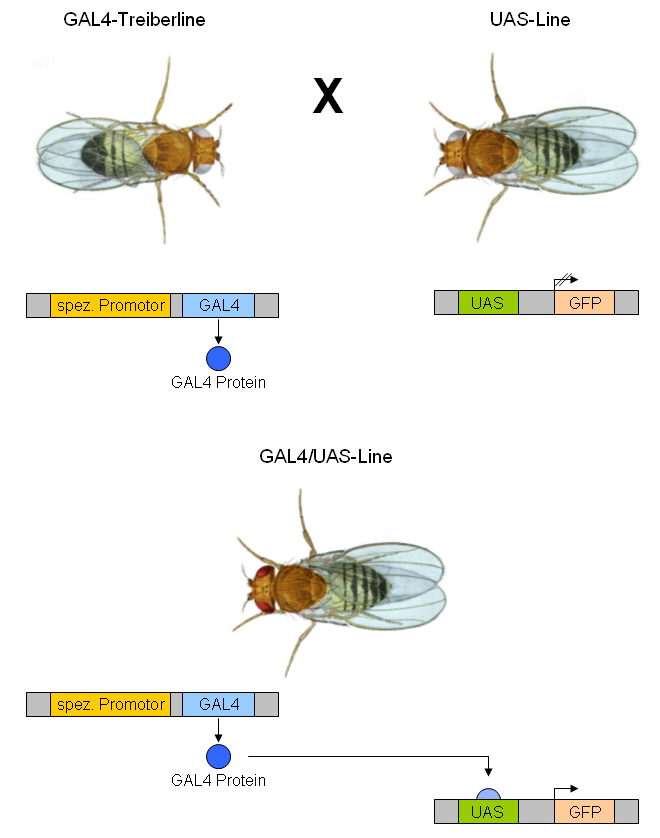
\includegraphics[width=0.7\textwidth]{lectures/160608/pix/Gal4UAS-System.png}
\end{center}

\underline{Effektor vs. Reporter}\\
 - Effektor: \\
 - Reporter: \\

\subsubsection{Modifikationen}

\textbf{Erweiterung durch GAL80}
\begin{itemize}
	\item kann als Repressor\footnote{\url{https://de.wikipedia.org/wiki/Repressor}} für GAL4 genutzt werden
	\item kann zusätzlich temperaturabhängig eingesetzt werden
\end{itemize}

\subsection{Was ist Lernen}
\begin{itemize}
	\item Lernen ist der Gedächtnis-bildende Prozess
\end{itemize}

\subsection{Assoziatives Lernen: Klassisches Konditionieren}
 - pawlowscher Hund\footnote{\url{https://de.wikipedia.org/wiki/Pawlowscher_Hund}}\\

\textbf{Wo im Gehirn findet Lernen statt?}
\begin{itemize}
	\item CS: conditioned stimulus (Glocke)
	\item US: unconditioned stimulus (Futter)
	\item UR: unconditioned response (Speicheln)
	\item CR: conditioned response (Speicheln)
\end{itemize}
\newpage
\textbf{CS-US Konvergenz-Punkt!}\\

\underline{Beispiel:} Kiemen-Rückziehreflexes von Aplysia
\begin{itemize}
	\item conditioned stimulus: taktiler Reiz
	\item unconditioned stimulus: Elektroschock
	\item unconditioned response: Kiemen-Rückziehreflexes
	\item conditioned response: Kiemen-Rückziehreflexes
	\item CS-US-Konvergenzpunkt: Motorneuron
\end{itemize}

\begin{center}
	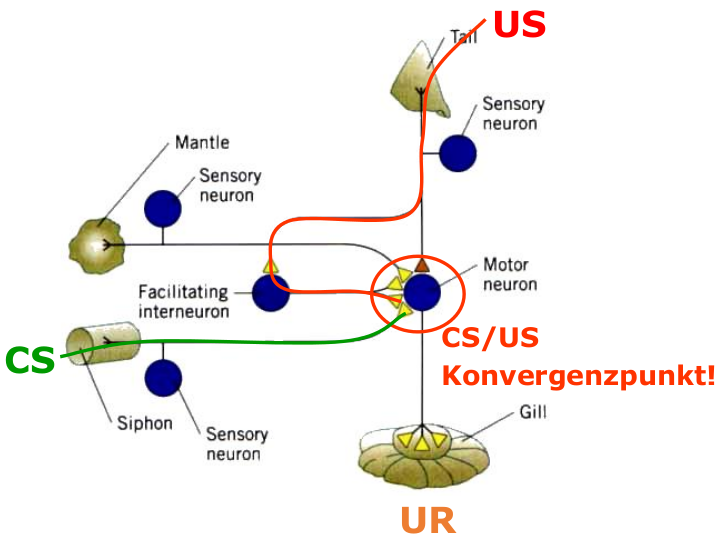
\includegraphics[width=0.7\textwidth]{lectures/160608/pix/cs_us_konvergenz.png}
\end{center}

\subsection{Molekulares Lernen}
 - Molekulare Konvergenz von CS und US! Koinzidenzdetektor\footnote{Koinzidenz ist ein zeitliches und/oder räumliches Zusammenfallen von Ereignissen oder Zusammentreffen von Objekten.}